% Copyright 2004 by Till Tantau <tantau@users.sourceforge.net>.
%
% In principle, this file can be redistributed and/or modified under
% the terms of the GNU Public License, version 2.
%
% However, this file is supposed to be a template to be modified
% for your own needs. For this reason, if you use this file as a
% template and not specifically distribute it as part of a another
% package/program, I grant the extra permission to freely copy and
% modify this file as you see fit and even to delete this copyright
% notice. 

\documentclass{beamer}

% There are many different themes available for Beamer. A comprehensive
% list with examples is given here:
% http://deic.uab.es/~iblanes/beamer_gallery/index_by_theme.html
% You can uncomment the themes below if you would like to use a different
% one:
%\usetheme{AnnArbor}
%\usetheme{Antibes}
%\usetheme{Bergen}
%\usetheme{Berkeley}
%\usetheme{Berlin}
%\usetheme{Boadilla}
%\usetheme{boxes}
%\usetheme{CambridgeUS}
%\usetheme{Copenhagen}
%\usetheme{Darmstadt}
%\usetheme{default}
%\usetheme{Frankfurt}
%\usetheme{Goettingen}
%\usetheme{Hannover}
%\usetheme{Ilmenau}
%\usetheme{JuanLesPins}
%\usetheme{Luebeck}
\usetheme{Madrid}
%\usetheme{Malmoe}
%\usetheme{Marburg}
%\usetheme{Montpellier}
%\usetheme{PaloAlto}
%\usetheme{Pittsburgh}
%\usetheme{Rochester}
%\usetheme{Singapore}
%\usetheme{Szeged}
%\usetheme{Warsaw}

\usepackage{amsmath}

\newcommand{\reels}{\mathbb{R}}
\newcommand{\norm}[1]{\left\lVert#1\right\rVert}

\title{Autoencoder a dimension reduction tool}


\author{Thomas LOUIS}
% - Give the names in the same order as the appear in the paper.
% - Use the \inst{?} command only if the authors have different
%   affiliation.

\date{2019}
% - Either use conference name or its abbreviation.
% - Not really informative to the audience, more for people (including
%   yourself) who are reading the slides online

% Let's get started
\begin{document}

\begin{frame}
  \titlepage
\end{frame}

\begin{frame}{Outline}
  \tableofcontents
  % You might wish to add the option [pausesections]
\end{frame}

% Section and subsections will appear in the presentation overview
% and table of contents.
\section{Dimension reduction}

\subsection{Dimensionality reduction}

\begin{frame}{Dimensionality reduction}{Optional Subtitle}
    Reducing dimensionality has several applications:
    \begin{itemize}
	    \item compressing data
	    \item coping with dimensionality curse
            \item denoising
    \end{itemize}
\end{frame}

\subsection{The PCA case}
\begin{frame}{The PCA case}
    Let's $M$ a ${N, d}$ matrix  of N vector $\in \reels^{d}$\\
    We wan't to find a projection base of subspace where variance of M is maximal \\
    $\hat{M}$ is the centred, normalized matrix of M \\
    $\hat{M}.\hat{M}'$ is diagonalizable thus $\hat{M}.\hat{M}' = P^{t}.\Delta.P$ \\
    $\Delta$ contains eigen vectors and P is the projection matrix for its eigenspace \\
    We only keep the eigen vectors that explain the most of the variance of M. \\
\end{frame}

\begin{frame}{The PCA case}
    PCA is able to catpure the linear relationships between correlated variables. \\
    example of applications: eigenfaces \\
    \begin{minipage}{6in}
    \centering
    $\vcenter{
    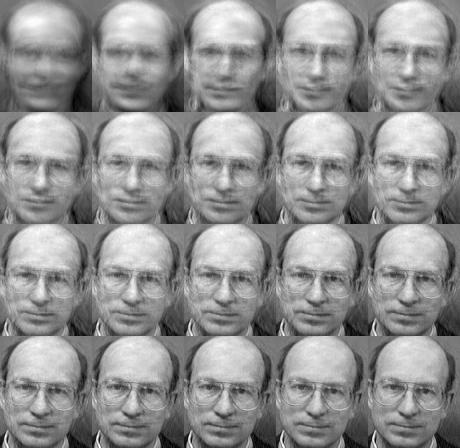
\includegraphics[scale=0.3]{data/eigenfaces.png}
    }$
    \end{minipage}
\end{frame}


\section{Autoencoder}
\subsection{Autoencoder architecture}
\begin{frame}{Autoencoder architecture}
    Autoencoder is a specific neural network architecture composed of:
    \begin{enumerate}
	\item an encoder network $f = \underset{i \in {{1 .. e}}}{O} L_i$
        \item a latent vector $h$
	\item a decoder network $g = \underset{i \in {{e + 1 .. d + e}}}{O} L_i$
    \end{enumerate}
    With $L_i : x \rightarrow \sigma(W_i.x + b)$ \\
    Where the input of the encoder has exactly the same dimensionality as the output of the decoder. \\
    \begin{minipage}{6in}
    \centering
    $\vcenter{
    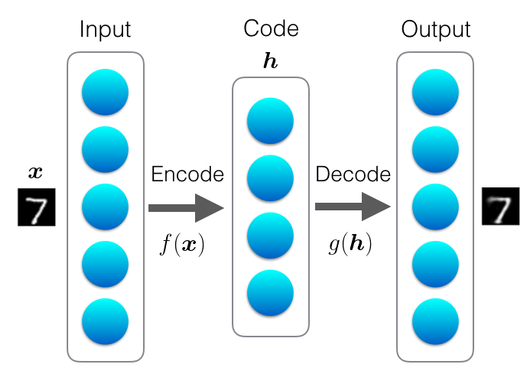
\includegraphics[scale=0.2]{data/autoencoder_illustration.png}
    }$
    \end{minipage}
\end{frame}

\subsection{Autoencoder optimization}
\begin{frame}{Autoencoder optimization}
	\begin{itemize}
		\item The output must reconstruct the input while having a bottleneck
		\item $(W_i)_{i \in {1 .. e+d}} = \underset{(W_i)_{i \in {1 .. e+d}}}{argmin} \norm{ x - f \circ g(x)}_f$
		\item Optimization is done using backpropagation algorithm
	\end{itemize}
\end{frame}

\subsection{Similarities with PCA}
\begin{frame}{Similarities with PCA}
	A linear autoencoder with one hidden layer is close to PCA\\
	We can rewrite $ f \circ g (x)$ as $A.B.x$ or $C.x$ with $C = A.B$\\
	then we want to optimize $\norm{ Y - C.X)}_f$ \\ 
	if $B = A^{t}$ we have $\norm{A^{t}.A - Y}_f = \norm{ P^t \Delta P. X - X}_f => ... $
\end{frame}

\begin{frame}{Similarities with PCA}
    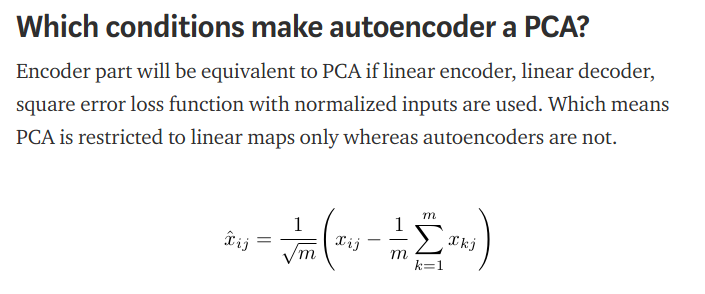
\includegraphics[scale=0.4]{data/pca_vs_autoencoder_bullshit1.png}
\end{frame}

\begin{frame}{Similarities with PCA}
    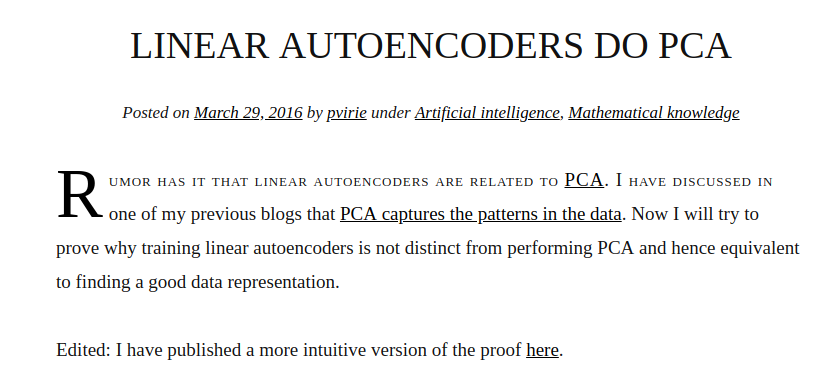
\includegraphics[scale=0.4]{data/pca_vs_autoencoder_bullshit2.png}
\end{frame}

\begin{frame}{Similarities with PCA}
	\begin{itemize}
		\item PCA : M' = S.M  
		\item AE : X = B.h
	\end{itemize}
We have close minimization objectives but orthogonality of $h$ is never ensured.
% dimensions in the projected subspace are totally uncorrelated in the first space
%
\end{frame}

\section{Variational Autoencoder}
\subsection{A Bayesian point of view}
\begin{frame}{Variational Autoencoder - A Bayesian point of view}
	We not only want to map one element to it's simbling with reduced representation, we want to learn distribution of the data
	$ p(x) = \int_\Omega p(x|t)p(t) dt$  \\
	With assumption: $p(t) = \mathcal{N}(0, I)$, 
	$ p(x| t) = \mathcal{N}(\mu(t),\,\Sigma(t))$ 
	
\end{frame}

% Placing a * after \section means it will not show in the
% outline or table of contents.
\section*{Summary}

\begin{frame}{Summary}
  \begin{itemize}
  \item
    The \alert{first main message} of your talk in one or two lines.
  \item
    The \alert{second main message} of your talk in one or two lines.
  \item
    Perhaps a \alert{third message}, but not more than that.
  \end{itemize}
  
  \begin{itemize}
  \item
    Outlook
    \begin{itemize}
    \item
      Something you haven't solved.
    \item
      Something else you haven't solved.
    \end{itemize}
  \end{itemize}
\end{frame}



% All of the following is optional and typically not needed. 
\appendix
\section<presentation>*{\appendixname}
\subsection<presentation>*{For Further Reading}

\begin{frame}[allowframebreaks]
  \frametitle<presentation>{For Further Reading}
    
  \begin{thebibliography}{10}
    
  \beamertemplatebookbibitems
  % Start with overview books.

  \bibitem{Author1990}
    A.~Author.
    \newblock {\em Handbook of Everything}.
    \newblock Some Press, 1990.
 
    
  \beamertemplatearticlebibitems
  % Followed by interesting articles. Keep the list short. 

  \bibitem{Someone2000}
    S.~Someone.
    \newblock On this and that.
    \newblock {\em Journal of This and That}, 2(1):50--100,
    2000.
  \end{thebibliography}
\end{frame}

\end{document}


